\documentclass[usenames,dvipsnames,12pt]{beamer}

\usetheme{Copenhagen}

\usepackage{tikz}
\usepackage{tkz-berge}
\usepackage{tkz-graph}
\usepackage{subcaption}
\usepackage{blkarray}
\usepackage{aligned-overset}
\usepackage{graphicx}
\usepackage{calc}

\setbeamertemplate{footline}[frame number]

\usetikzlibrary{patterns,arrows,decorations.pathreplacing}

\usepackage{xcolor}
\definecolor{dblue}{RGB}{20,66,129}
\definecolor{rose}{RGB}{255,101,122}
\definecolor{crimsonred}{RGB}{132,22,23}
\definecolor{darkblue}{RGB}{72,61,139}

\definecolor{deepblue}{RGB}{36,123,160}
\definecolor{deepred}{RGB}{255,22,84}
\definecolor{deeporange}{RGB}{240,111,62}

\definecolor{olive}{rgb}{0.3, 0.4, .1}
\definecolor{fore}{RGB}{249,242,215}
\definecolor{back}{RGB}{51,51,51}
\definecolor{title}{RGB}{255,0,90}
\definecolor{dgreen}{rgb}{0.,0.6,0.}
\definecolor{gold}{rgb}{1.,0.84,0.}
\definecolor{JungleGreen}{cmyk}{0.99,0,0.52,0}
\definecolor{BlueGreen}{cmyk}{0.85,0,0.33,0}
\definecolor{RawSienna}{cmyk}{0,0.72,1,0.45}
\definecolor{Magenta}{cmyk}{0,1,0,0}

\DeclareMathOperator{\QQ}{\mathbf{Q}}
\DeclareMathOperator{\ZZ}{\mathbb{Z}}
\DeclareMathOperator{\RR}{\mathbb{R}}
\DeclareMathOperator{\HH}{\mathbf{H}}
\DeclareMathOperator{\CC}{\mathbf{C}}
\DeclareMathOperator{\AB}{\mathbf{A}}
\DeclareMathOperator{\PP}{\mathbb{P}}
\DeclareMathOperator{\MM}{\mathbf{M}}
\DeclareMathOperator{\VV}{\mathbf{V}}
\DeclareMathOperator{\TT}{\mathbf{T}}
\DeclareMathOperator{\LL}{\mathcal{L}}
\DeclareMathOperator{\EE}{\mathbb{E}}
\DeclareMathOperator{\NN}{\mathbf{N}}
\DeclareMathOperator{\DQ}{\mathcal{Q}}
\DeclareMathOperator{\IA}{\mathfrak{a}}
\DeclareMathOperator{\IB}{\mathfrak{b}}
\DeclareMathOperator{\IC}{\mathfrak{c}}
\DeclareMathOperator{\IP}{\mathfrak{p}}
\DeclareMathOperator{\IQ}{\mathfrak{q}}
\DeclareMathOperator{\IM}{\mathfrak{m}}
\DeclareMathOperator{\IN}{\mathfrak{n}}
\DeclareMathOperator{\IK}{\mathfrak{k}}
\DeclareMathOperator{\ord}{\text{ord}}
\DeclareMathOperator{\Ker}{\textsf{Ker}}
\DeclareMathOperator{\Coker}{\textsf{Coker}}
\DeclareMathOperator{\emphcoker}{\emph{coker}}
\DeclareMathOperator{\pp}{\partial}
\DeclareMathOperator{\tr}{\text{tr}}

\newtheorem*{goal}{Goal}



\title{Nodal Domains and Diffusion Processes}
\author{Jacob Denson}

\institute{University of Wisconsin Madison}

\begin{document}

\maketitle

\begin{frame}

\begin{itemize}
    \item Georgiev, Mukherjee, \emph{Nodal Geometry, Heat Diffusion, and Brownian Motion}, Anal. PDE. {\bf 12} (2017), 133-148.
    \pause

    \item Steinerberger, \emph{Lower Bounds on Nodal Sets of Eigenfunctions via the Heat Flow}, Comm. Partial Differential Equations. {\bf 39} (2014), 2240-2261.
    \pause

    \item {\O}ksendal, \emph{Stochastic Differential Equations}, Springer, 2003.

    \item Chung, \emph{Green, Brown, and Probability and Brownian Motion}, World Scientific Publishing Company, 2002.
\end{itemize}

\end{frame}

\begin{frame}
    \frametitle{Nodal Domains}

    % Write Notation on Board
    \begin{goal}
        Study `asymptotic geometry' of $D_\lambda$ as $\lambda \to \infty$.
    \end{goal}

    \pause

    \vspace{20pt}

    \begin{center}
        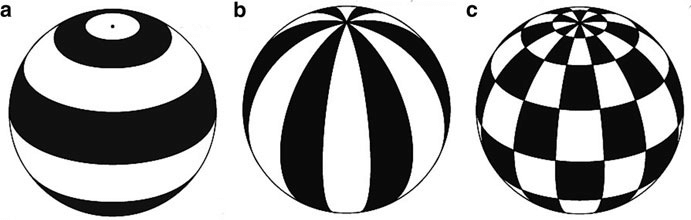
\includegraphics[scale=0.3]{zonalsectorialtesseralharmonics.png}

        \hspace*{10pt}\hbox{\scriptsize Credit:\thinspace{\small\itshape \scriptsize Yuri Skiba}}
    \end{center}

%        \item Let $(M^d,g)$ be a compact Riemannian manifold.
%        \item Let $e_\lambda \in C^\infty(M)$, $\Delta_g e_\lambda = - \lambda^2 e_\lambda$.
%        \item \emph{Nodal Set} of $e_\lambda$: $Z_\lambda = \{ x \in M: e_\lambda(x) = 0 \}$.
%        \item \emph{Nodal Domain} $D_\lambda$: a connected component of $M - Z_\lambda$.

        % TODO: Add Pictures

        % lambda = sqrt(l(l+1))
        % Separation of Variables: e_lambda(theta,psi) = Theta(theta) Phi(phi)
        
        % Zonal Harmonic: P_l(cos theta). Zeroes are roughly spaced at a distance O(1/l) = O(1/lambda) apart.
        % Roots of P_l are approximately (1 - 1/8n^2) cos(pi k/n)

        % Also spaced a distance O(1/lambda) apart

        % Tesseral: P^m_l(cos theta) cos(m phi)
        % |m| <= lambda
        % Again, observe O(1/lambda) thickness boxes.
\end{frame}

\begin{frame}
    \frametitle{Nodal Domains}

    \begin{center}
        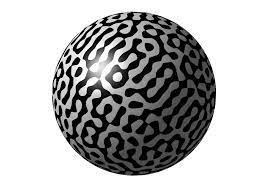
\includegraphics[scale=0.6]{lowdegreesphericalharmonic.jpg}
        \hspace{10pt}
        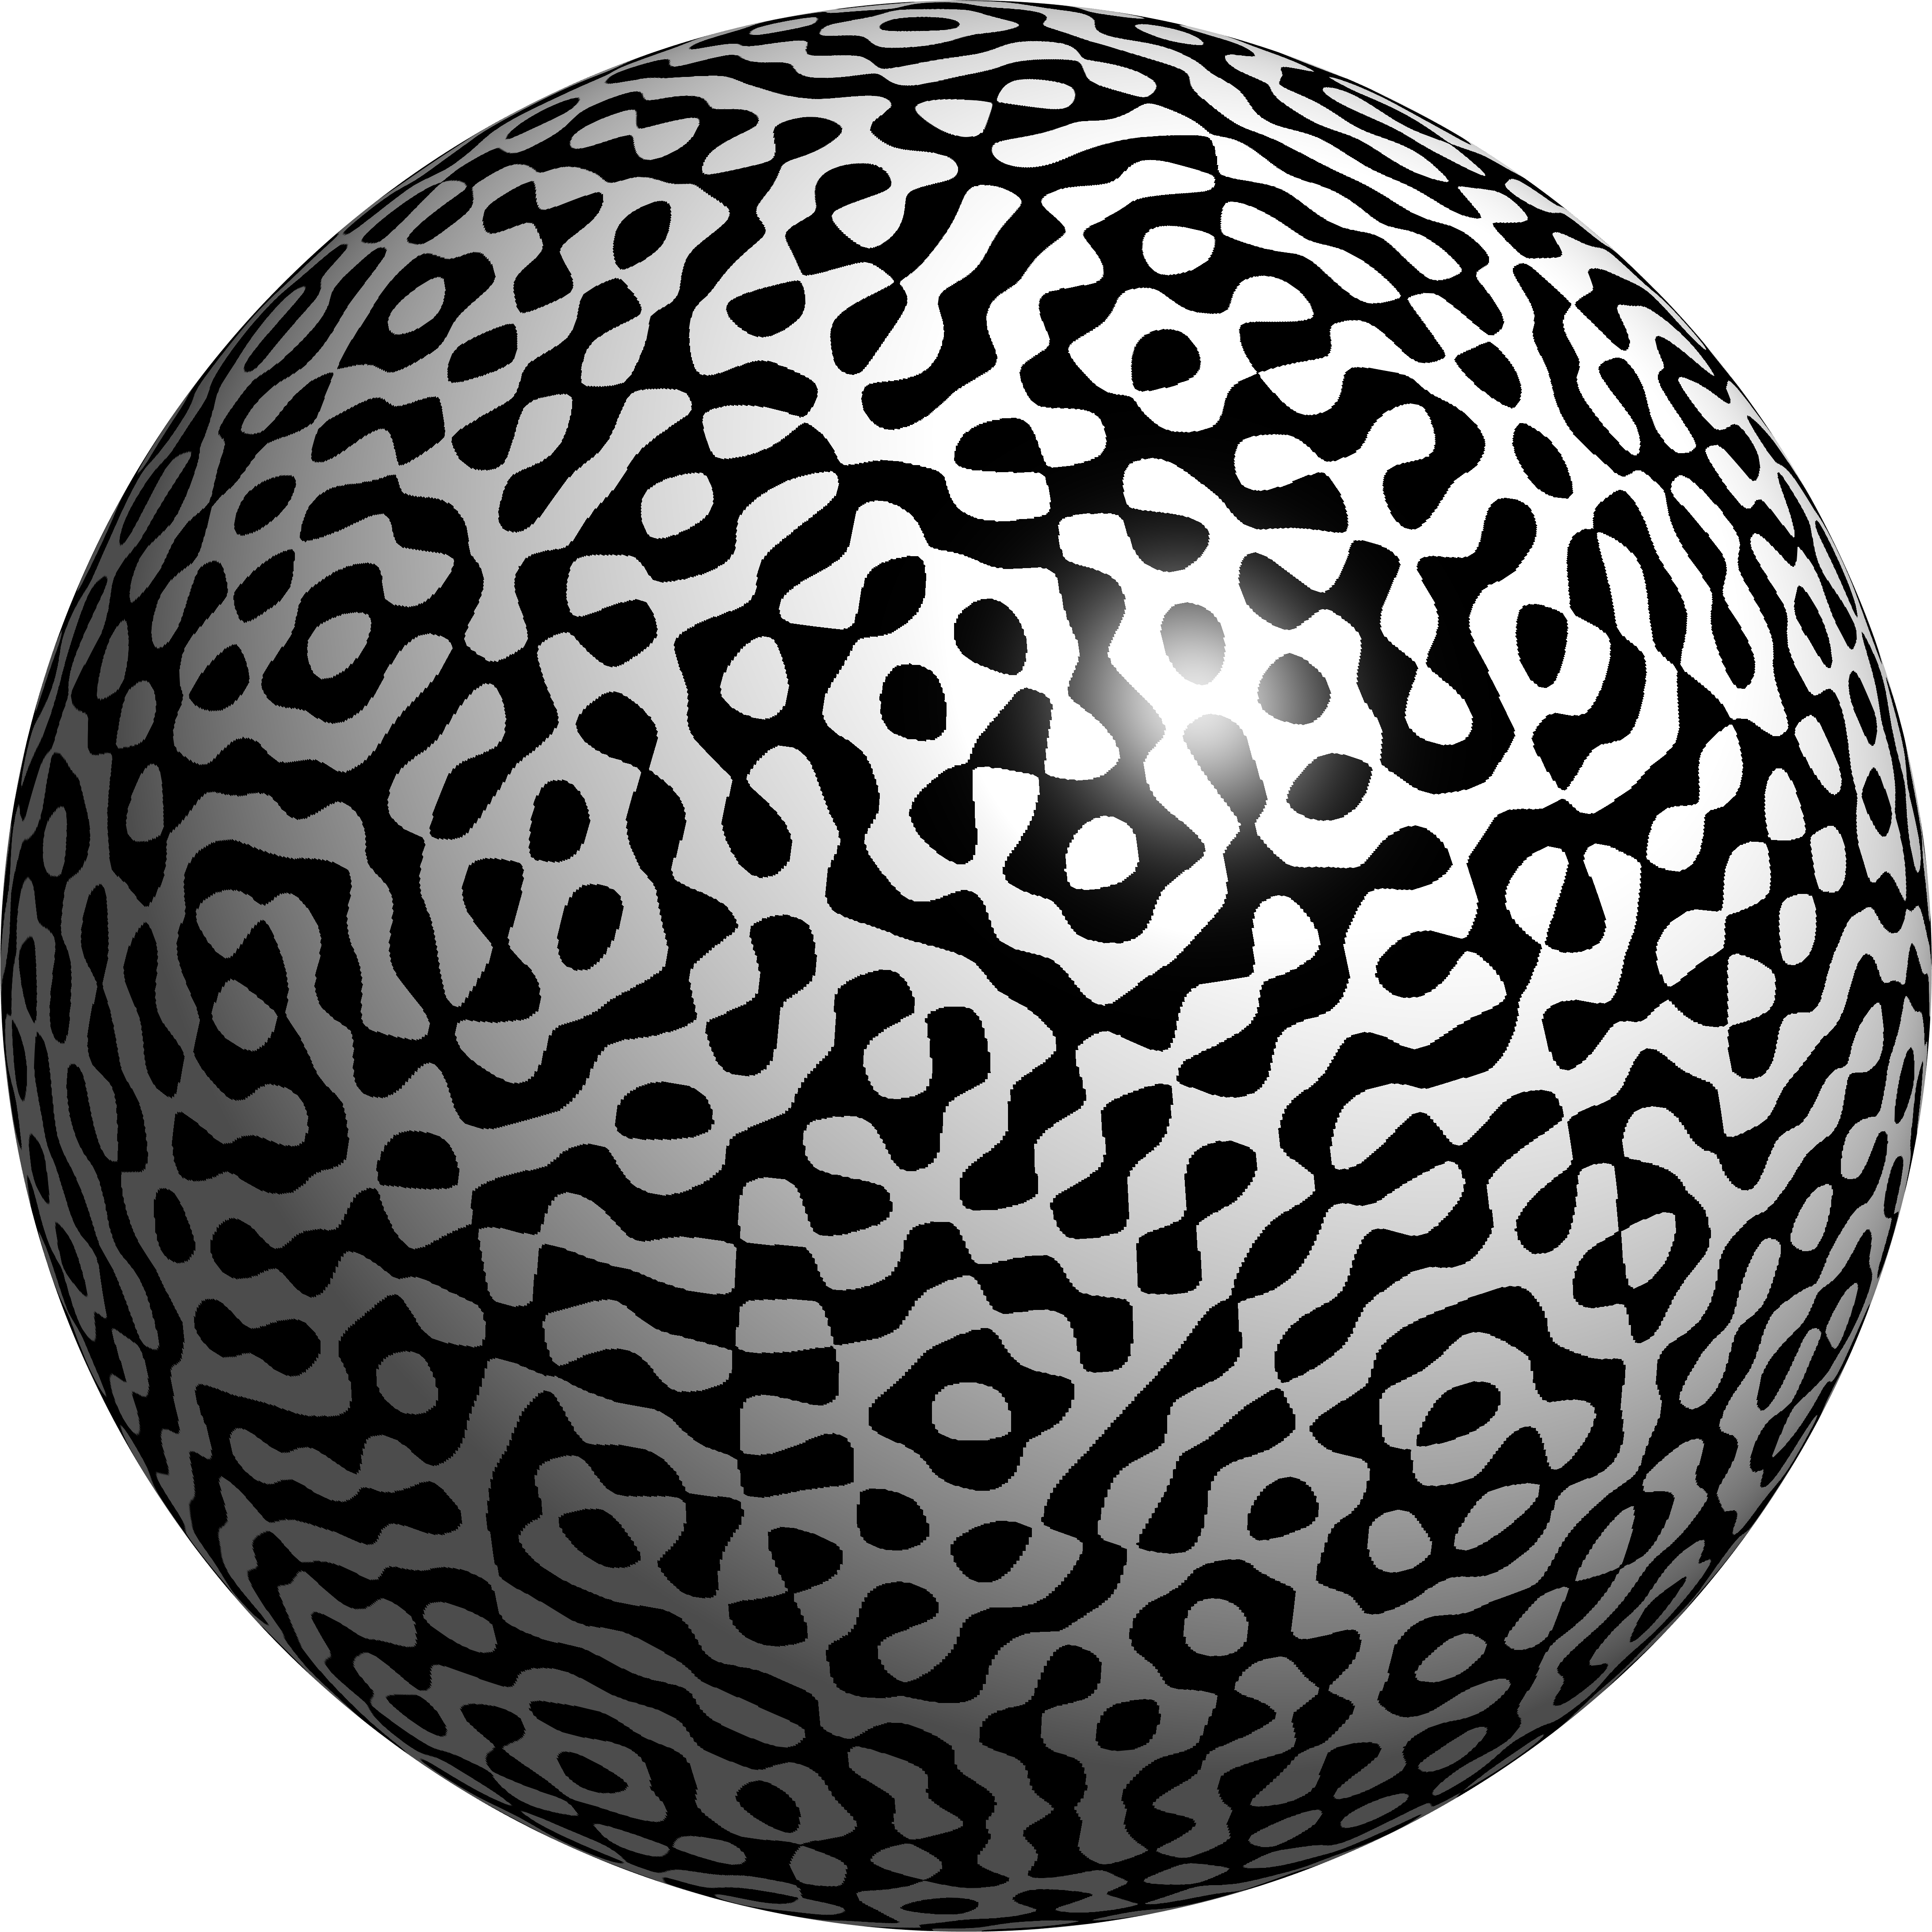
\includegraphics[scale=0.6]{highdegreesphericalharmonic.png}

        \hspace*{10pt}\hbox{\scriptsize Credit:\thinspace{\small\itshape \scriptsize Alex Barnett}}
    \end{center}

%        \item Let $(M^d,g)$ be a compact Riemannian manifold.
%        \item Let $e_\lambda \in C^\infty(M)$, $\Delta_g e_\lambda = - \lambda^2 e_\lambda$.
%        \item \emph{Nodal Set} of $e_\lambda$: $Z_\lambda = \{ x \in M: e_\lambda(x) = 0 \}$.
%        \item \emph{Nodal Domain} $D_\lambda$: a connected component of $M - Z_\lambda$.

        % TODO: Add Pictures

        % lambda = sqrt(l(l+1))
        % Separation of Variables: e_lambda(theta,psi) = Theta(theta) Phi(phi)
        
        % Zonal Harmonic: P_l(cos theta). Zeroes are roughly spaced at a distance O(1/l) = O(1/lambda) apart.
        % Roots of P_l are approximately (1 - 1/8n^2) cos(pi k/n)

        % Also spaced a distance O(1/lambda) apart

        % Tesseral: P^m_l(cos theta) cos(m phi)
        % |m| <= lambda
        % Again, observe O(1/lambda) thickness boxes.
\end{frame}

\begin{frame}
    \frametitle{Main Result}

    \begin{itemize}
        \item {\bf Theorem}: There is $c_M > 0$ such that for any `good' $k$-dimensional submanifold $\Sigma$ of $M$, then
        %
        \[ N(\Sigma, c_M / \lambda) = \{ x \in M : d(x,\Sigma) < c_M / \lambda \} \]
        %
        \emph{doesn't contain} $D_\lambda$.

        \pause
        \item Consider the radius $1/\lambda$ tubular neighborhood
        %
        \[ T_{1/\lambda} \Sigma = \bigcup\nolimits_{x \in \Sigma} \{ v \in (T_x \Sigma)^\perp: |v|_g \leq 1/\lambda \}. \]
        %
        The submanifold $\Sigma$ is `good' if the geodesic map $T_{1/\lambda} \Sigma \to N(\Sigma, 1/\lambda)$ is an embedding.
        % So we have `tubular coordinates' on $N(\Sigma, 1/\lambda)$.
        % Take geodesic examples on torus

        \pause
        \begin{itemize}
            \item Local condition: All principal curvatures of $\Sigma$ are $\lesssim \lambda$.

            \pause
            \item But no cheating globally!
            % TODO: Think about this
            % After Injectivity Radius, all bets are off 
        \end{itemize}
    \end{itemize}
\end{frame}

\begin{frame}
    \frametitle{Main Result}

    \begin{itemize}
        \item {\bf Theorem}: There is $c_M > 0$ such that for any `good' $k$-dimensional submanifold $\Sigma$ of $M$, then
        %
        \[ N(\Sigma, c_M / \lambda) = \{ x \in M : d(x,\Sigma) < c_M / \lambda \} \]
        %
        \emph{doesn't contain} $D_\lambda$.

%        \item Can replace $\Sigma$ with a finite union of $\Omega(1/\lambda)$ separated `good' submanifolds. Or allow finite unions with `transverse enough' intersections.

        \pause
        \item There is $C_M > 0$ such that $D_\lambda \subset N(Z_\lambda, C_M/\lambda)$, contrasting this result.

        \pause
        \item Proof Heuristic: Elliptic methods tend to give $O(1/\lambda)$ localized results. We study stochastic diffusions, which provide cool tools for analyzing eigenfunctions from an elliptic perspective!
        % TODO: Find citation
    \end{itemize}
\end{frame}

\begin{frame}
    \frametitle{Uncertainty Principle Type Thing?}

    \begin{itemize}
        \item What would an analogous result look like on $\RR^d$?
        \pause

        \item {\bf Theorem}: Let $D_\lambda$ be a nodal domain in $\RR^d$. Then there is $c_d > 0$ such that if $\Sigma$ is a finite union of $O(1/\lambda)$-separated $k$ dimensional planes, then $D_\lambda$ is not contained in $N(\Sigma, c_d / \lambda)$.
        \pause

        \item Stronger Result: $D_\lambda$ should contain a ball of radius $O(1/\lambda)$ by the uncertainty principle.

        % ASK TOMORROW: DO WE HAVE BOUNDS ON THE MAXIMUM VALUE OF AN EIGENFUNCTION ON A NODAL DOMAIN?
        % We have D^alpha f(x) <= lambda^{|alpha|} |f|_{L^infty}

        \pause
        \item Version on Manifolds: Paper also proves that $D_\lambda$ contains `a large percentage' of a ball of radius $O(1/\lambda)$ using similar techniques.

        \pause
        \item Related Methods: $D_\lambda$ satisfies an `interior cone condition' with angle $O(1/\lambda)$.
%        for any $\varepsilon_0 > 0$, there is $r_0 > 0$ such that if $x^* = \text{argmax}_{x \in D_\lambda} \{ e_\lambda(x) \}$, then $D_\lambda$ contains $1 - \varepsilon_0$ percent of $B(x_0,r_0 \lambda^{-1/2})$.
    \end{itemize}
\end{frame}

\begin{frame}
    \frametitle{Continuous Stochastic Processes}

    \begin{itemize}
        \item Three ways to view continuous stochastic processes:

        \begin{itemize}
            \pause
            \item As Borel-measurable functions
            %
            \[ X: \Omega \to C([0,\infty), M). \]

            \pause
            \item As a family of correlated random variables
            %
            \[ \{ X_t: \Omega \to M : t \in [0,\infty) \}. \]

            \pause
            \item As a law predicting future behaviour from present behaviour, i.e. by defining quantities such as
            %
            \[ \EE^x[f(X)] = \EE[f(X) | X_0 = x]. \]
        \end{itemize}
    \end{itemize}
\end{frame}

\begin{frame}
    \frametitle{Brownian Motion on $\RR^d$}

    \begin{itemize}
        \item Brownian motion is a stochastic process $\{ B_t \}$ such that:
        \pause

        \begin{itemize}
            \item For any $I = [t,s]$, given $B_t = x$, the random variable $\Delta_I B = B_s - B_t$ is normally distributed with mean $x$ and variance $s - t$.

            \pause
            \item For any family of disjoint intervals $I_1,\dots,I_N \subset [0,\infty)$, with $I_k = [t_k,s_k]$, the random variables $\Delta_{I_k} B$ are independent from one another.
        \end{itemize}
    \end{itemize}

    \vspace{-5pt}

    \begin{center}
        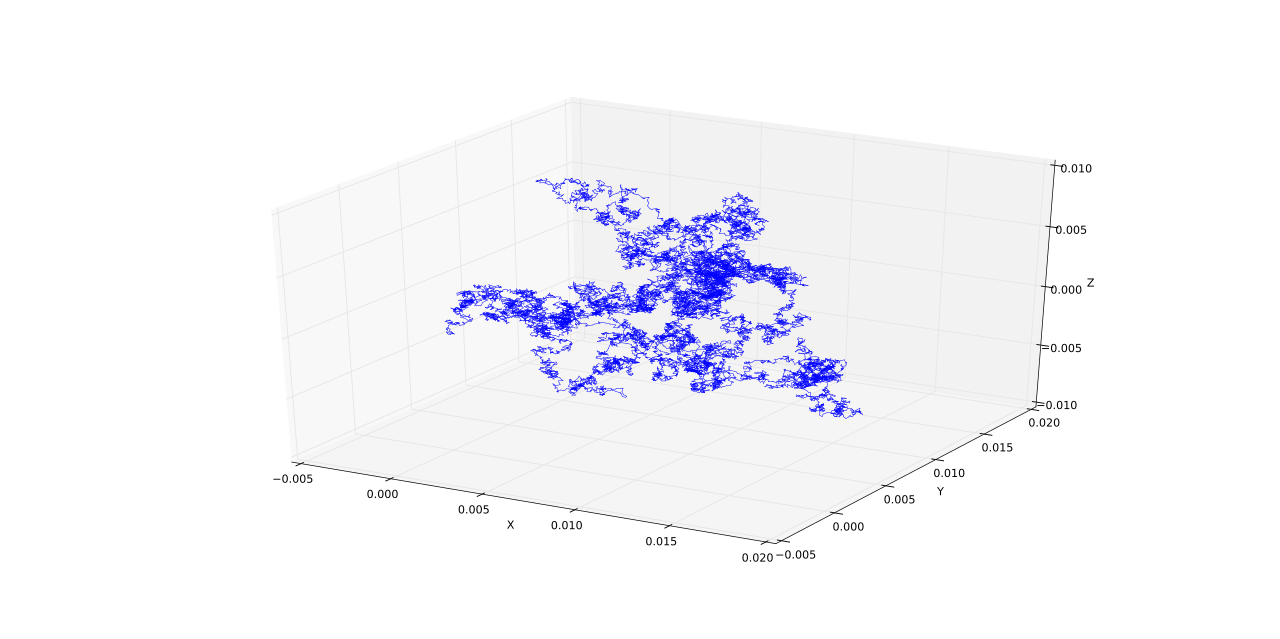
\includegraphics[scale=0.2]{BrownianMotion.png}

        \vspace{-15pt}
        \hspace*{10pt}\hbox{\scriptsize Credit:\thinspace{\small\itshape \scriptsize Shiyu Ji}}
    \end{center}
\end{frame}

\begin{frame}
    \frametitle{It\^{o} Diffusions}

    \begin{itemize}
        \item An It\^{o} Diffusion is like Brownian Motion, but diffusion is not radially symmetric.

        \pause
        \item For each $x \in \RR^d$, let $A(x)$ be a $d \times d$ positive semidefinite matrix. Then we have an It\^{o} diffusion $\{ X_t \}$ given in law by the `Stochastic differential equation' $dX = A(X) dB$.

        \pause
        \item For practical purposes, we have
        %
        \[ X_{t + \delta} - X_t \approx A(X_t) [B_{t + \delta} - B_t] \]
        % X_delta = A(x) B_delta
        % Ball of radius delta^{1/2} stretched in direction
        %
        where the difference between the LHS and RHS is a random variable with mean $o(\delta)$, and variance $O(\delta)$. %L^3$ norm $O(\delta)$.

        \pause
        \item Diffuses locally near $x$ faster in directions where $A(x)$ has large eigenvalues.
    \end{itemize}

    % TODO: Picture of Ito diffusion
\end{frame}

% Tr(A^T H A) = (Delta/2)(f)
\begin{frame}
    \frametitle{It\^{o} Diffusions}

    \begin{itemize}
        \item Can define It\^{o} diffusions on compact Riemannian manifolds $M$ given a section $A: M \to \text{Hom}(TM)$ of positive definite matrices.

        \pause
        \item We can define Brownian motion on a Riemannian manifold such that Brownian motion diffuses at a unit speed along geodesics.
    \end{itemize}

    \begin{center}
        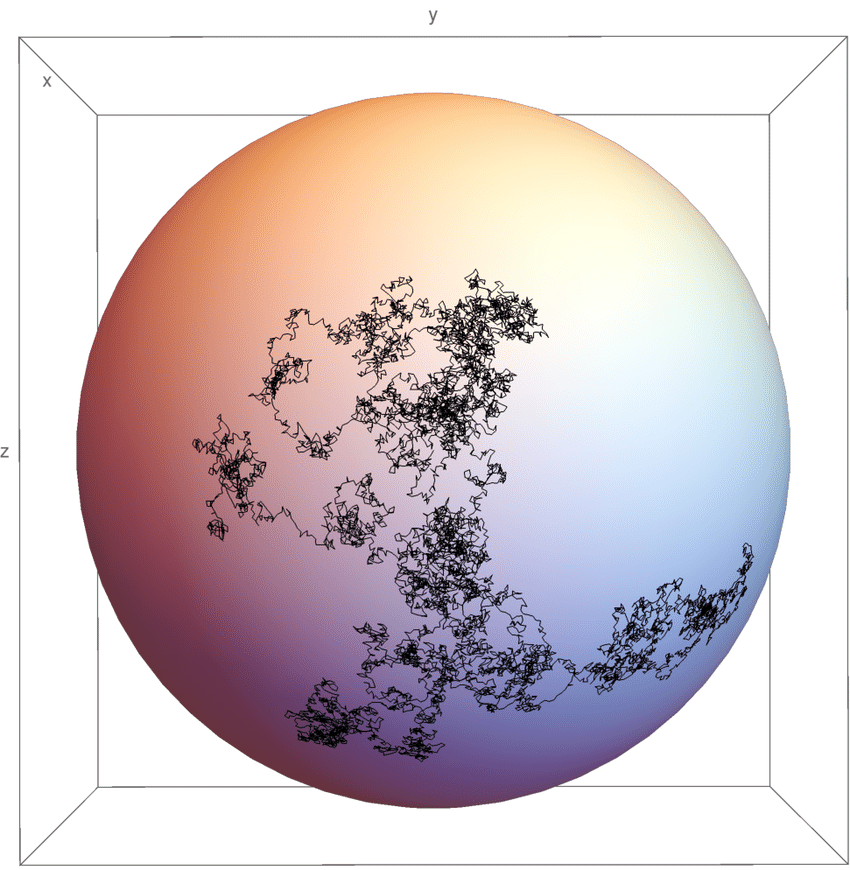
\includegraphics[scale=0.1]{BrownianMotionSphere.png}

        \hspace*{10pt}\hbox{\scriptsize Credit:\thinspace{\small\itshape \scriptsize Ma, Matveev, Pavlyukevich}}
    \end{center}
\end{frame}





\begin{frame}
    \frametitle{Connection to Elliptic Operators}

    \begin{itemize}
        \item For any diffusion $X$, we can associate a semielliptic operator $L$, the \emph{generator} of $X$, such that for $f \in C^\infty(M)$,
        %
        \begin{align*}
            Lf(x) &= \left. \partial_t \{ \EE^x[f(X_t)] \} \right|_{t = 0} = \lim_{t \to 0^+} \frac{\EE^x[f(X_t)] - f(x)}{t}.
        \end{align*}

        \pause
        \item Second order because paths of $X$ are `half differentiable'.

        \pause
        \item For Brownian motion (on $\RR^d$ or a manifold $M$), $L = \Delta / 2$.

        \pause
        \item `Morally' apply the Fundamental Theorem of Calculus to get \emph{Dynkin's Formula}
        %
        \[ \EE^x[f(X_T)] = f(x) + \EE^x \left[ \int_0^T (Lf)(X_s)\; ds \right]. \]
    \end{itemize}
\end{frame}





\begin{frame}
    \frametitle{Application: Escape Times}

    \begin{itemize}
        \item In Dynkin's formula, $T$ can be a `stopping time', i.e. any $[0,\infty)$ valued function of $X$ which doesn't `predict the future', i.e. if $T$ stops at a time $t$, it must only stop because of the properties of $X$ on $[0,T]$, and not behaviour on $(T,\infty)$.

        \pause
        \item Given an open, bounded set $U$, let
        %
        \[ T_U = \inf \{ t : X_t \not \in U \} \]
        %
        be the \emph{escape time} of $U$.

        \pause
        \item If $B$ is Brownian motion on $\RR^d$, and $U$ is the escape time of a ball of radius $R^{1/2}$ centered at $x$, $\EE^x[T_U] = R / n$.

        \pause
        \item If $B$ is Brownian motion on $M$, escape time will be slower if volume expands (negative curvature) and faster if volume contracts (positive curvature). This is irrelevant for the values $R = O(1/\lambda)$ that we care about.
        % (Delta / 2) f(y) = n + 2r partial_r det(d exp_p) / det(d exp_p)
        % exp_p(q + tv) = q + tv + O(r^2)
        % d exp_p(q) = I + O(r^2)
        % det(d exp_p) = det(I + O(r^2)) = 1 + O(r^2)
        % O(r^2)
        % r^2 = E[ int_0^T [n + O(r^2)] ] = ( n + O(r^2) ) E^x[T]
        % E^x[T] = r^2 / ( n + O(r^2) )
        % Up to the times we care about, essentially flat.
    \end{itemize}
\end{frame}





\begin{frame}
    \frametitle{Feynman Kac Formula}

    \begin{itemize}
        \item Reverses Dynkin's Formula: Solves PDEs via Diffusions.

        \pause
        \item Physically Intuitive Situations:
        \begin{itemize}
            \pause
            \item (1) If $\partial_t u = Lu$ on $M$ with $u_0 = f$, then
            %
            \[ u(x,t) = \EE^x[f(X_t)]. \]

            \pause
            \item (2) $\partial_t u = Lu$ on $D \subset M$ with $u_0 = f$ and $u = 0$ on $\partial M$,
            %
            \[ u(x,t) = \EE^x[f(X_t) \chi_t], \]
            %
            where $\chi_t = \mathbb{I}(T_D > t)$ \emph{kills} paths absorbed by $\partial D$.

            \pause
            \item (3) If $Lv = 0$ on $D \subset M$ with $v = \phi$ on $\partial D$, then
            %
            \[ v(x) = \EE^x \left[ \phi(X_{T_D}) \right]. \]

            \pause
            \item Can also solve $\partial_t u = Lu$ with $\partial u / \partial \eta = 0$ on $\partial D$ using `reflection on Brownian motion', but a little more technical with singularities.
        \end{itemize}
    \end{itemize}
\end{frame}



\begin{frame}
    \frametitle{The Proof}

    And now, back to our regularly scheduled programming

    \begin{itemize}
        \item {\bf Theorem}: There is $c_M > 0$ such that for any `good' $k$-dimensional submanifold $\Sigma$ of $M$, then
        %
        \[ N(\Sigma, c_M / \lambda) = \{ x \in M : d(x,\Sigma) < c_M / \lambda \} \]
        %
        \emph{doesn't contain} $D_\lambda$.

        \pause
        \item Assume $e_\lambda \geq 0$ on $D_\lambda$. Let $x^* = \text{argmax} \{ e_\lambda(x) \}$.

        \pause
        \item Let $p(x,t)$ and $u(x,t)$ solve $\partial_t = \Delta$ with initial / boundary conditions:
        %
        \begin{itemize}
            \item $p_0 = 0$ and $p = 1$ on $\partial D_\lambda$.
            \item $u_0 = e_\lambda$, and $u = 0$ on $\partial D_\lambda$.

            \pause
            \item $p(x,t) = \PP^x(T_D \geq t | X_0 = x)$.
            \item $u(x,t) = \EE[e_\lambda(B_t) \chi_t]$.
        \end{itemize}

        % v = 1
        % p - v equals -1 initially
        % f = 0
        %

        % Feynman-Kac,
        % p(x,t) = 1 - \EE^x[ chi_T ] = P(Tau <= t).
        % u(x,t) = E^x[ e_lambda(B_t) chi_T ] = e^{- lambda^2 t} e_lambda(x)

        % Thus e^{-lambda^2 t} e_lambda(x) = u(x,t) = E^x[e_lambda(B_t) chi_T] <= e_lambda(x^*) E^x[chi_T] = e_lambda(x_0) (1 - p(x,t))
        % Thus if x = x^*, p(x^*,t) <= 1 - e^{-lambda^2 t}
        % Thus the probability of exiting D after time O(1/lambda^2) starting at x^* is small.
        % Thus x^* must be O(1/lambda) from the boundary

        % Have precise conditions on the probability of exiting D in *euclidean case*.
        % Since time is small, Euclidean case is comparable to Riemannian case.
    \end{itemize}
\end{frame}

\begin{frame}
    \frametitle{Thanks For Listening!}
\end{frame}

% Capacity is related to chance Brownian motion enters a set.
% Used to prove Euclidean is comparable to Riemannian

\end{document}